% Search for all the places that say "PUT SOMETHING HERE".

\documentclass[11pt]{article}
\usepackage{amsmath,textcomp,fancyvrb,pdfpages, amssymb,geometry,graphicx,enumerate,bm,hyperref}
\graphicspath{ {images/} }

\title{CS189--FALL 2015 --- Homework 4 Write up}
\author{ZUBO GU, SID 25500921, gu.zubo@berkeley.edu}
\markboth{}{}
\pagestyle{myheadings}
\date{}

\begin{document}
\maketitle

\section*{Problem 1. solution}
\begin{itemize}
\item[a].
$J(\textbf{w},\omega_0) = (\textbf{y - Xw} - \omega_0 \textbf{1})^T(\textbf{y - Xw} - \omega_0 \textbf{1}) + \lambda \textbf{w}^T\textbf{w}$

=$\textbf{y}^T\textbf{y} - \textbf{y}^T\textbf{Xw} - \textbf{y}^T\omega_0\textbf{1} - \textbf{w}^T\textbf{X}^T\textbf{y} +  \textbf{w}^T\textbf{X}^T\textbf{XW}  + \textbf{w}^T\textbf{X}^T\omega_0\textbf{1} + \textbf{1}^T\omega_0 y+ \textbf{1}^T\omega_0 \textbf{XW} +
\omega_0^2 \textbf{1}^T\textbf{1} + \lambda \textbf{w}^T\textbf{w}$

derivative with respect to $\omega_0$ and set equal to 0, we get

$-y^T1 + w^TX^T1 - 1^Ty+1^TXw + 2\omega_01^T1 = 0$

$X^T1 = 0$ since $\overline{x}= 0,  1^T1 = n$

$-\sum_{i=1}^{n} y_i  -\sum_{i=1}^{n} y_i + 2 \omega_0 n = 0$

Thus, $\omega_o = \frac{1}{n} \sum_{i=1}^{n} y_i = \overline{y}$ which is optimal.

derivative with respect to $\textbf{w}$ and set equal to 0, we get

$-x^Ty - x^Ty + 2 X^TXw + X^T\omega_0 + X^T\omega_0 1 + 2\lambda I w = 0$

Simplify, $(X^TX + \lambda I)w = X^Ty$
Thus, $ w= (X^TX + \lambda I)^{-1}X^Ty$ which is optimal.

\item[b].
\begin{itemize}

\item[i].
code see attach q1.py

\item[ii].
The RSS is 6.03013493e+13

The residuals sum of squares increase compare to HW3 result.

\item[iii].
The 1st, 7th an 8th coefficients are still most significant. However, comparing to HW3 result, 
The 1st coefficient value increase in magnitude
The 7th an 8th coefficients value decrease magnitude.

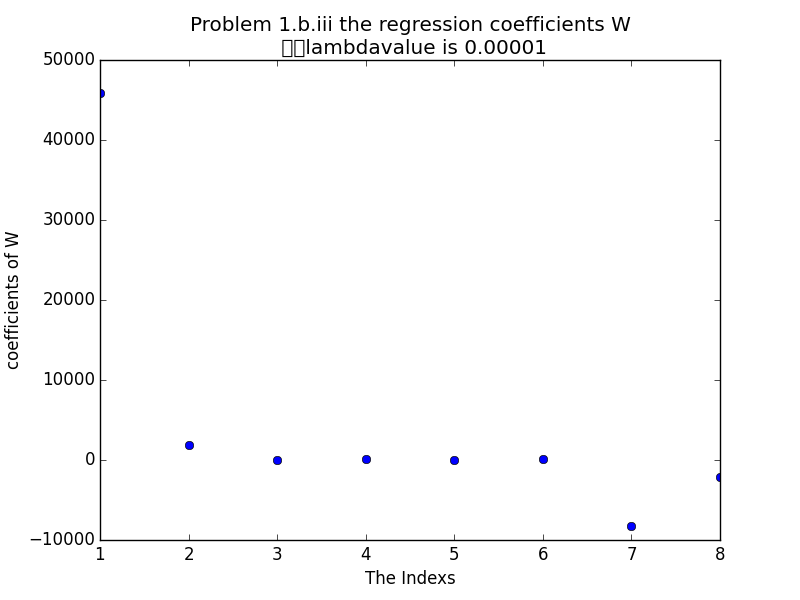
\includegraphics[scale=0.6]{q1}

\end{itemize}
\end{itemize}


\section*{Problem 2. solution}
\begin{itemize}

\item[a].
$\frac{1}{36}$

\item[b].

$1 - (1 - \frac{1}{36}) ^ 6 = \frac{3781}{46656}$

\item[c].

\item[d].
No. the $\alpha = 0.05 /5 = 0.01$. Thus, we can't assert "significant better" that with 5 percent wrong. 

\item[e].
$p = 1 - (1 - {p}')^m$

$ (1 - p)^{\frac{1}{m}} = 1 - {p}'$ 

$ {p}' = 1 - (1 - p)^{\frac{1}{m}} = 1 - (1 - \frac{p}{m}) = \frac{p}{m}$ as p is very small

Thus, $p = m * {p}'$ the Bonferroni correction

\item[f].
P(at least one significant result) = $1 - (1 - 0.0001)^{50000} = 0.99326373738$. Thus it is a significant gene. 

By computer the Bonferroni correction we get 0.0001 * 50000 = 5 which is greater than 1. Because we have large number test which make the result 


\end{itemize}


\section*{Problem 3. solution}
\begin{itemize}
\item[a].
There are four possible cases $P(X, Y) \in \lbrace (0,1), (0, -1), (1, 0), (-1, 0) \rbrace$

$E(X) = E(Y) =  \frac{1}{4} * -1 + 0 * \frac{1}{2} + \frac{1}{4} * 1 = 0$

$E(XY) = 0$ since there is one zero between X Y for all possible cases.

Thus, $COV(X,Y) = E(XY) - E(X) E(Y) = 0$, X and Y are uncorrelated.

 $P(X = 0,Y = 1) = \frac{1}{4}$. But, $P(X = 0) = \frac{1}{2},P(Y = 1) = \frac{1}{4}$
 
Thus, $ P(X, Y) \neq P(X)P(Y)$, X and Y are not independent.
\item[b].

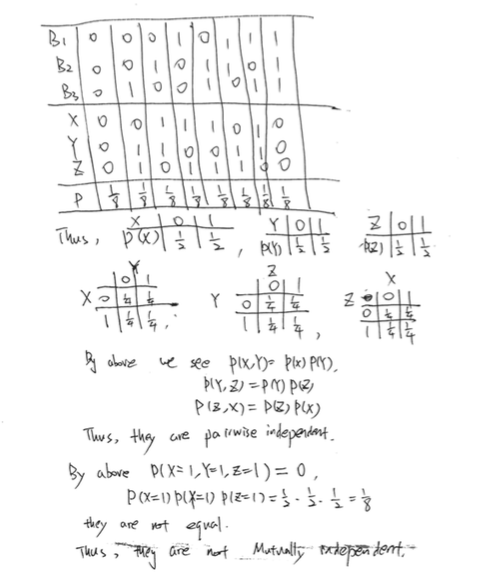
\includegraphics[scale=0.6]{q32}

\item[c].

The good features should be uncorrelated to each other. Thus, when we have redundant that are correlated to another feature, we can eliminate it and reduce the computation of data. 

Thus, for data set that all features are independent. we can't eliminate feature
\end{itemize}

\newpage
\section*{Problem 4. solution}

\begin{itemize}
\item[a].

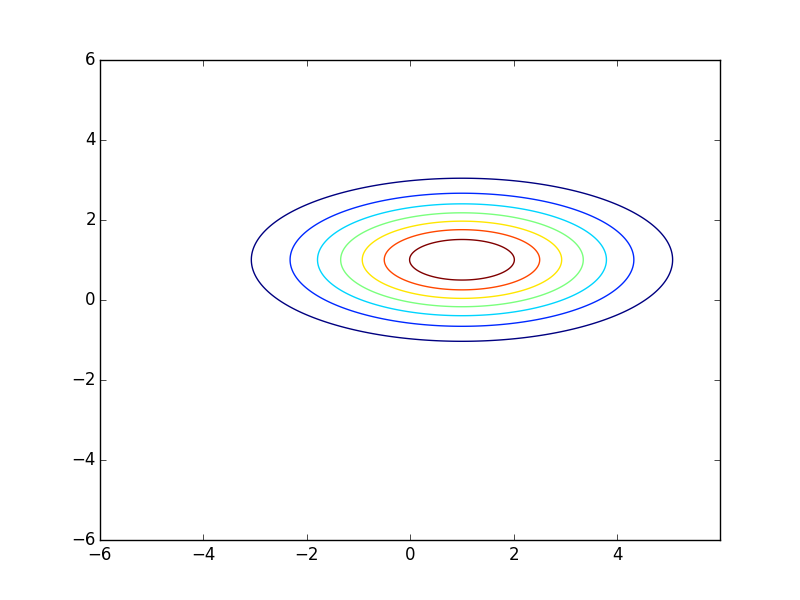
\includegraphics[scale=0.55]{q41}

\item[b].

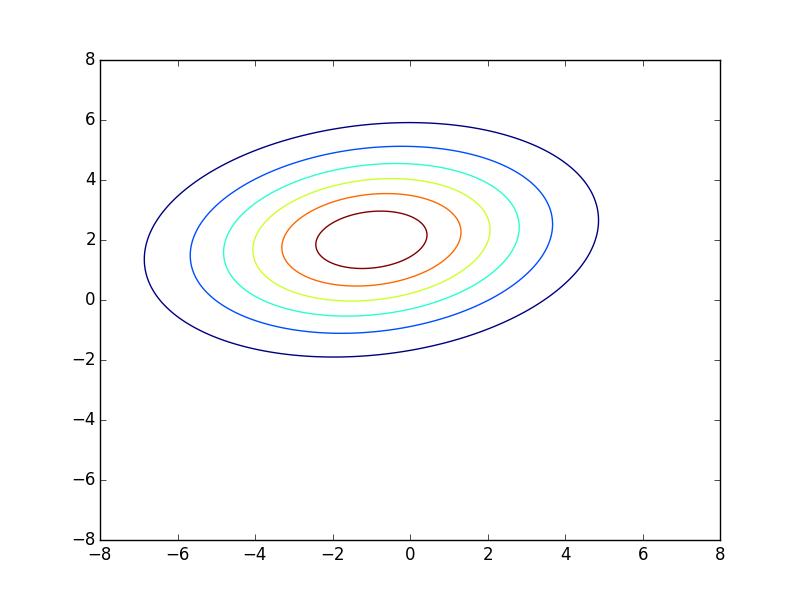
\includegraphics[scale=0.55]{q42}

\item[c].

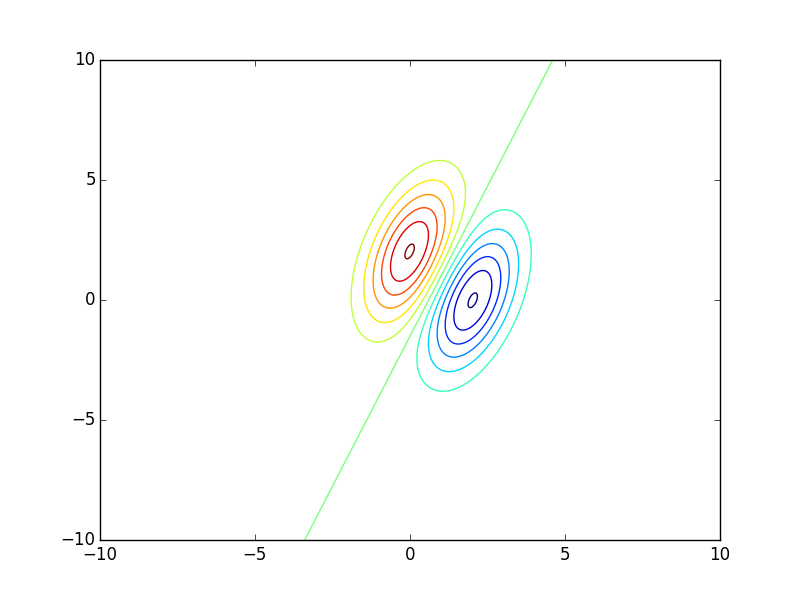
\includegraphics[scale=0.55]{q43}
\item[d].

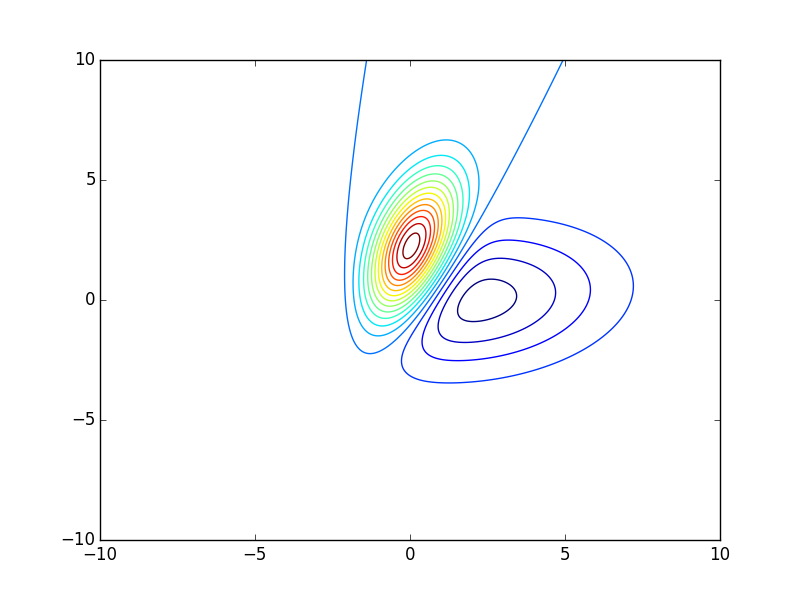
\includegraphics[scale=0.55]{q44}
\item[e].

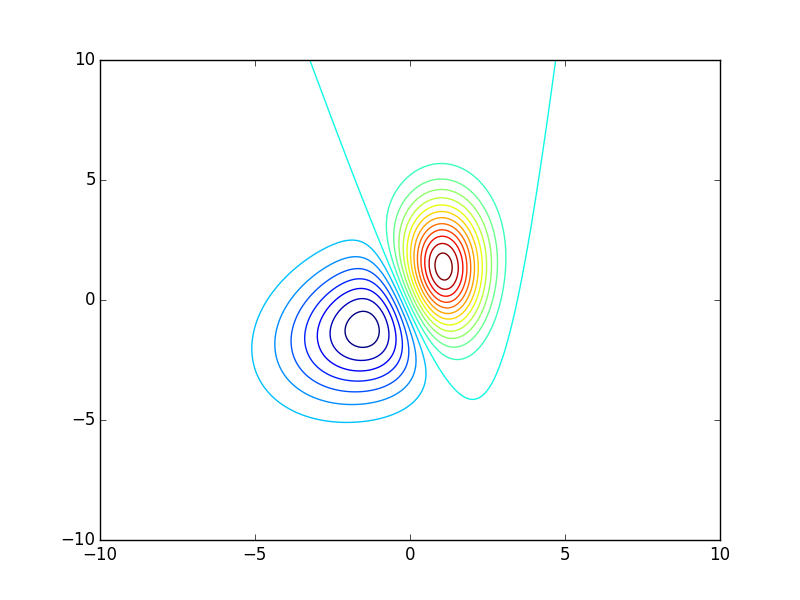
\includegraphics[scale=0.55]{q45}
\end{itemize}

\section*{Problem 5. solution}
\begin{itemize}
\item[a].

part.a. mean of X1 is 2.67187421622

part.a. mean of X2 is 5.33879004655

\item[b].

 convaranceMatrix is 
 [[ 7.54570894  3.8874626 ]
 [ 3.8874626   5.90007162]]

\item[c].

eeigenvalue is  10.6964775788 eigenvector is  [ 0.77687579  0.62965387]
eigenvalue is  2.74930298331 eigenvector is  [-0.62965387  0.77687579]

\item[d].

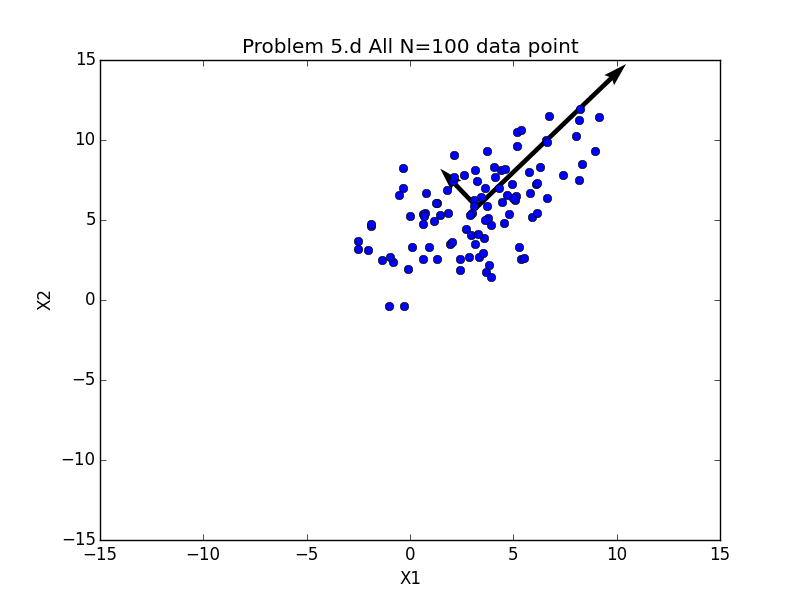
\includegraphics[scale=0.55]{q54}

\item[e].

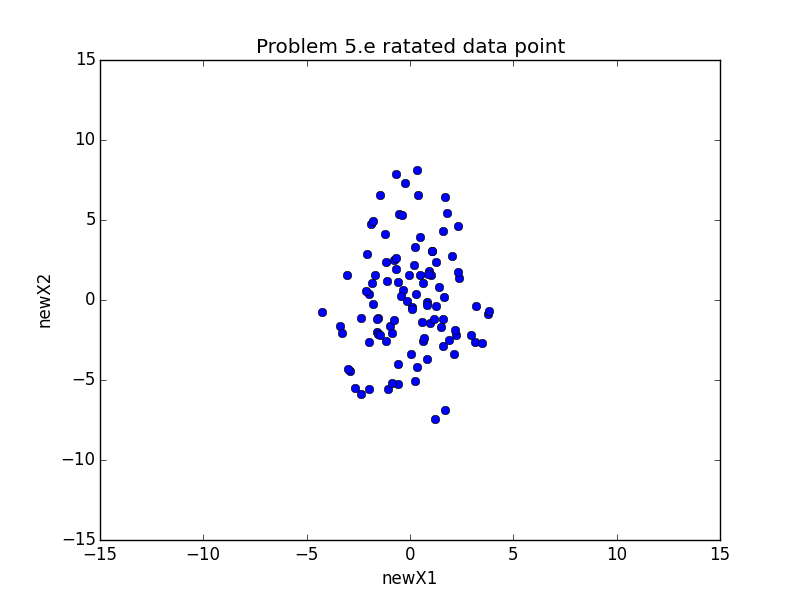
\includegraphics[scale=0.55]{q55}

\end{itemize}

\section*{Problem 6. solution}
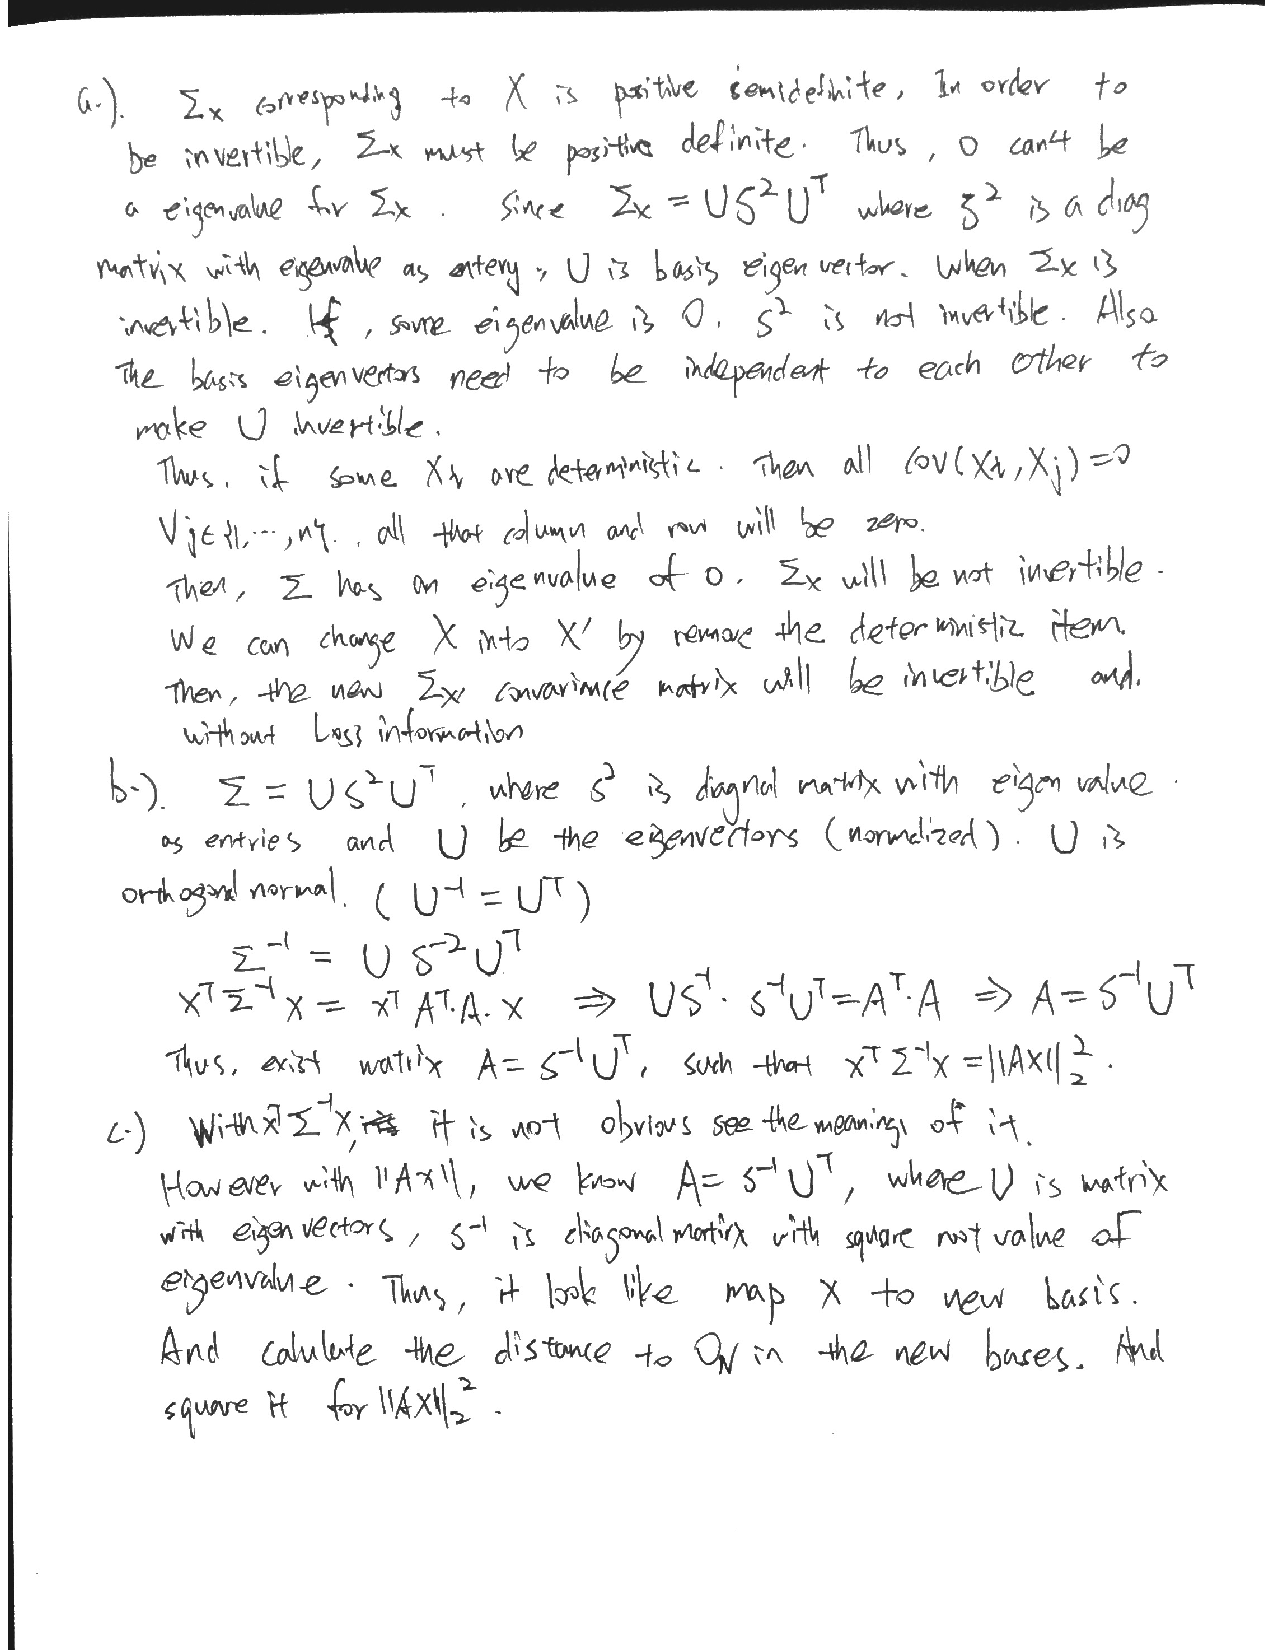
\includepdf[pages=-]{q6.pdf}

\section*{Problem 7. solution}
\begin{itemize}
\item[a].

means $\mu =  \frac{1}{n}\sum_{i=1}^{n} y_i$

covariance matrices $\Sigma = \frac{1}{n }\sum_{i=1}^{n}(X_i - \mu)^T(X_i - \mu)$

Model see $q7\cdot py$
\item[b].
Compute the size for each class in the train data the divide by the total size of the train data which is the prior probability for that class

The prior probability for  0 is 0.09871666666666666

The prior probability for  1 is 0.11236666666666667

The prior probability for  2 is 0.0993

The prior probability for  3 is 0.10218333333333333

The prior probability for  4 is 0.09736666666666667

The prior probability for  5 is 0.09035

The prior probability for  6 is 0.09863333333333334

The prior probability for  7 is 0.10441666666666667

The prior probability for  8 is 0.09751666666666667

The prior probability for  9 is 0.09915
\item[c].
Below is visualize picture for digit 2.In the center area, some positive value in diagonal, left-bottom and right top, some negative value around diagonal. Zeros are in four edges.

This is 784 x 784 matrix, as we concatenate 28 * 28 matrix to a 784 x 1 row vector. thus, most part of this graph is zero, since they are 0 in the row vector. Only original term not 0, we can get a covariance not zero. Thus,center area has same nonzero value since they are related and could be nonzero in the center of a 28 * 28 matrix. The edges in original  28 x 28 are most zeros, too.

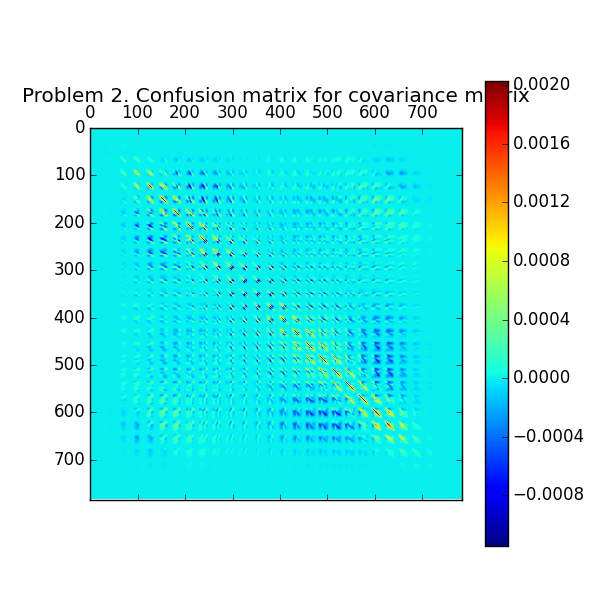
\includegraphics[scale=0.5]{q73}
\item[d].
\begin{itemize}
\item[i].

For here, the decision boundary is linear since we share the same covariance matrix. 

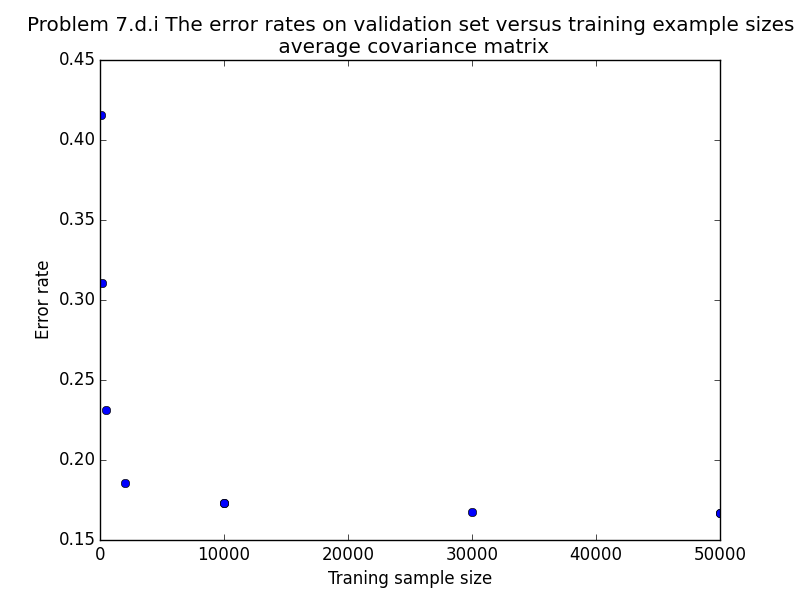
\includegraphics[scale=0.5]{q741}

\item[ii].
For here, the decision boundary is quadratic  since each class has their own covariance matrix. 

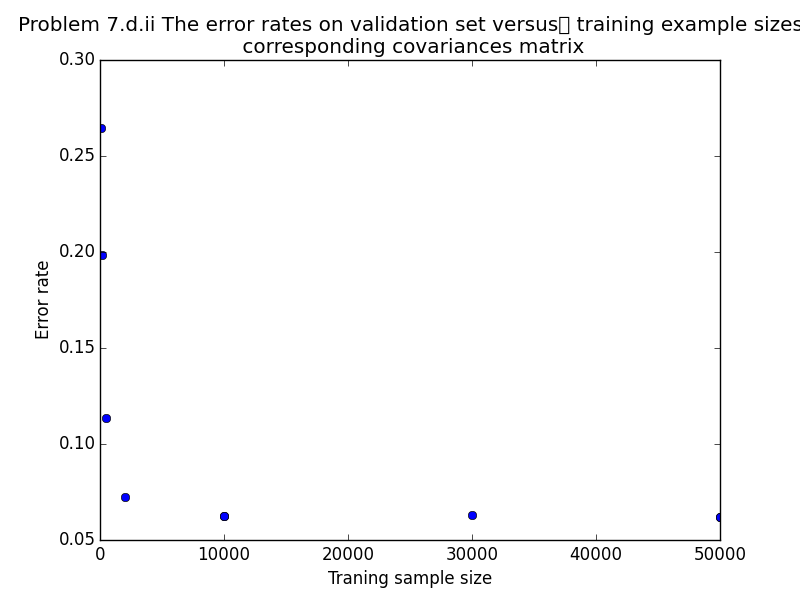
\includegraphics[scale=0.5]{q742}
\item[iii].
The second method is lower in error rate which mean more accuracy in predict performance. Since second method does not using average covariance matrix and the decision boundary is quadratic, it will be more accuracy in making right predicts. 

\item[iv].
Optimal prediction rate is 0.94600

\end{itemize}
\item[e]. Optimal prediction rate is 0.73506

\end{itemize}

\newpage
\section*{q1 code}
\VerbatimInput[baselinestretch=1,fontsize=\footnotesize,numbers=left]{q1.py}

\newpage
\section*{q4 code}
\VerbatimInput[baselinestretch=1,fontsize=\footnotesize,numbers=left]{q4.py}

\newpage
\section*{q5 code}
\VerbatimInput[baselinestretch=1,fontsize=\footnotesize,numbers=left]{q5.py}

\newpage
\section*{q7 code}
\VerbatimInput[baselinestretch=1,fontsize=\footnotesize,numbers=left]{q7.py}

\newpage
\section*{q7 for kaggle digit code}
\VerbatimInput[baselinestretch=1,fontsize=\footnotesize,numbers=left]{q7_d_iv.py}

\newpage
\section*{q7 for kaggle digit code}
\VerbatimInput[baselinestretch=1,fontsize=\footnotesize,numbers=left]{q7_e.py}

\end{document}


